
\documentclass[journal,12pt,twocolumn]{IEEEtran}
\usepackage[none]{hyphenat}
\usepackage{graphicx}
\usepackage{listings}
\usepackage[english]{babel}
\usepackage{graphicx}
\usepackage{caption} 
\usepackage{amsmath}
\usepackage{hyperref}
\usepackage{booktabs}
\usepackage{array}


\title{\textbf{\\Assignment on line}}
\author{Sireesha Abbavaram - FWC22060}
\begin{document}
\maketitle


\section{Question}
\textbf{\textit{Class 11, Exercise 10.1, Q(6):} Without using the pythagoras theorem ,show that the points (4,4),(3,5) and (-1,-1) are the vertices of a right angled triangle.}

\begin{figure}[h!]
\centering
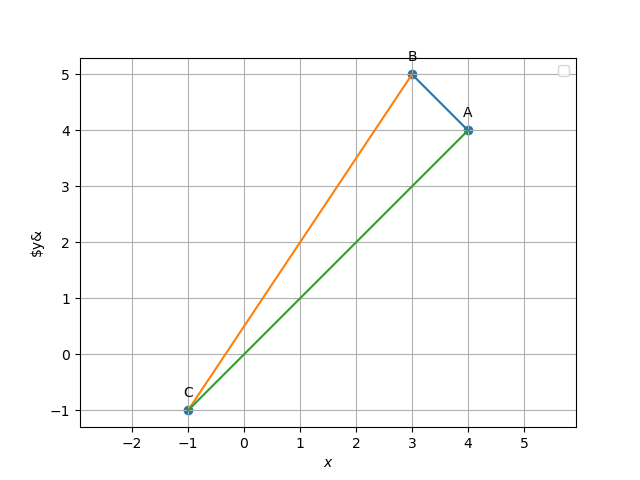
\includegraphics[scale=0.35]{triangle.png}
\centering
\caption{Traingle ABC}
\end{figure}


\section{Solution}
\raggedright 
\vspace{0.25cm}
Let A,B and C be the vertices of a given traingle with coordinates $\begin{pmatrix}
4 \\
4
\end{pmatrix}
, \begin{pmatrix}
3 \\
5
\end{pmatrix}
 and \begin{pmatrix}
-1 \\
-1
\end{pmatrix} $
\raggedright
. we have verify whther the given vertices are of right angled triangle or not.\\
\begin{center}
\raggedright
Let The directional vector of two vectors A and B is given as AB (m1)=A-B.
\end{center}
\vspace{0.25cm}
\begin{center}
The directional vector of the vectors B and C is given as BC (m2)=B-C.
\end{center}
\vspace{0.25cm}
\begin{center}
The directinal vector of the vectors C and A is given as CA (m3)=C-A.
\end{center}
\vspace{0.25cm}
The angle between any two vectors is given by
\boldmath
\\ $ cos b =\frac{(m1)^T(m2)}{||m1|| ||m2||}  equation-1$
\unboldmath
\vspace{0.5cm}\raggedright\\
Where b is the angle between the two vectors .
when the angle b=90 ,we get cos 90=0.
\vspace{0.5cm}\raggedright\\
It implies that the numerator of the equation 1 should be zero.

\vspace{0.25cm}
 In order to prove that the triangle is right angled we have to show any two vectors should be orthogonal to each other.
 
\vspace{0.25cm}\raggedright
So we need to show $(A-B)^T(B-C) or (B-C)^T(C-A) or (C-A)^T(A-B) $ is equal to zero.

\vspace{0.5cm}\raggedright
C-A=$\begin{pmatrix}
-1 \\
-1 
\end{pmatrix}
-\begin{pmatrix}
4 \\
4 \
\end{pmatrix}
=\begin{pmatrix}
-5 \\
-5 \
\end{pmatrix}$
\vspace{0.5cm}\raggedright\\
$(C-A)^T=(-5\space -5),$
\vspace{0.5cm}\raggedright
A-B=$\begin{pmatrix}
4 \\
4 \ 
\end{pmatrix}
-\begin{pmatrix}
3 \\
5 \
\end{pmatrix}
=\begin{pmatrix}
1 \\
-1 \
\end{pmatrix}$
\vspace{0.25cm}\raggedright
$(C-A)^T(A-B)=(-5 -5)\begin{pmatrix}
1 \\
-1 \
\end{pmatrix}
=-5+5=0$
\vspace{0.25cm}\raggedright
From above we can say that directional vectors CA and AB are perpendicular to each other.\\
\vspace{0.25cm}\raggedright
Thus we have right angle at the vertex A.


\vspace{0.2cm}
\section*{Construction}
\centering
\vspace{0.2cm}
{
\setlength\extrarowheight{2pt}
\begin{tabular}{|c|c|c|}
	\hline
	\textbf{Symbol}&\textbf{Value}&\textbf{Description}\\
	\hline
	A & (4,4) & Vertex A\\
	\hline
	B & (3,5) & Vertex B\\
	\hline
	C & (-1,-1) & Vertex C\\
	\hline
	
\end{tabular}
}

\vspace{0.6cm}
Get the python code of the figures from
\begin{table}[h]
\large
\centering
\begin{tabular}{|l|}
\hline
https://github.com/Sireesha1602/sireesha/
\\blob/main/line assignment \\
\hline
\end{tabular}

\end{table}




\end{document}
